% questions.tex —— 2013 年·湖南卷·文科 · 题目内容片段（无答案）
% 由 tools/generate_projects.py 依来源总账自 2013/2013_数学真题_湖南文_试题.md 生成，勿手改（改源 MD 后重跑）
\gkpart{一、选择题}
\begin{question}
\gkti{1}复数 $z=\mathrm i\cdot(1+\mathrm i)$（$\mathrm i$ 为虚数单位）在复平面上对应的点位于\mbox{（　　）}
（A）第一象限；（B）第二象限；（C）第三象限；（D）第四象限。
\end{question}
\begin{question}
\gkti{2}“$1<x<2$”是“$x<2$”成立的\mbox{（　　）}
（A）充分不必要条件；（B）必要不充分条件；（C）充分必要条件；（D）既不充分也不必要条件。
\end{question}
\begin{question}
\gkti{3}某工厂甲、乙、丙三个车间生产了同一种产品，数量分别为 $120$ 件，$80$ 件，$60$ 件。为了解它们的产品质量是否存在显著差异，用分层抽样方法抽取了一个容量为 $n$ 的样本进行调查，其中从丙车间的产品中抽取了 $3$ 件，则 $n=$\mbox{（　　）}
（A）$9$；（B）$10$；（C）$12$；（D）$13$。
\end{question}
\begin{question}
\gkti{4}已知 $f(x)$ 是奇函数，$g(x)$ 是偶函数，且 $f(-1)+g(1)=2$，$f(1)+g(-1)=4$，则 $g(1)$ 等于\mbox{（　　）}
（A）$4$；（B）$3$；（C）$2$；（D）$1$。
\end{question}
\begin{question}
\gkti{5}在锐角 $\triangle ABC$ 中，角 $A$，$B$ 所对的边长分别为 $a$，$b$。若 $2a\sin B=\sqrt3b$，则角 $A$ 等于\mbox{（　　）}
（A）$\dfrac\pi3$；（B）$\dfrac\pi4$；（C）$\dfrac\pi6$；（D）$\dfrac\pi{12}$。
\end{question}
\begin{question}
\gkti{6}函数 $f(x)=\ln x$ 的图象与函数 $g(x)=x^2-4x+4$ 的图象的交点个数为\mbox{（　　）}
（A）$0$；（B）$1$；（C）$2$；（D）$3$。
\end{question}
\begin{question}
\gkti{7}已知正方体的棱长为 $1$，其俯视图是一个面积为 $1$ 的正方形，侧视图是一个面积为 $\sqrt2$ 的矩形，则该正方体的正视图的面积等于\mbox{（　　）}
（A）$\dfrac{\sqrt3}2$；（B）$1$；（C）$\dfrac{\sqrt2+1}2$；（D）$\sqrt2$。
\end{question}
\begin{question}
\gkti{8}已知 $\boldsymbol a$，$\boldsymbol b$ 是单位向量，$\boldsymbol a\cdot\boldsymbol b=0$。若向量 $\boldsymbol c$ 满足 $|\boldsymbol c-\boldsymbol a-\boldsymbol b|=1$，则 $|\boldsymbol c|$ 的最大值为\mbox{（　　）}
（A）$\sqrt2-1$；（B）$\sqrt2$；（C）$\sqrt2+1$；（D）$\sqrt2+2$。
\end{question}
\begin{question}
\gkti{9}已知事件“在矩形 $ABCD$ 的边 $CD$ 上随机取一点 $P$，使 $\triangle APB$ 的最大边是 $AB$”发生的概率为 $\dfrac12$，则 $\dfrac{AD}{AB}=$\mbox{（　　）}
（A）$\dfrac12$；（B）$\dfrac14$；（C）$\dfrac{\sqrt3}2$；（D）$\dfrac{\sqrt7}4$。
\end{question}
\gkpart{二、填空题}
\begin{question}
\gkti{10}已知集合 $U=\{2,3,6,8\}$，$A=\{2,3\}$，$B=\{2,6,8\}$，则 $(\complement_U A)\cap B=$\gkblank{}。
\end{question}
\begin{question}
\gkti{11}在平面直角坐标系 $xOy$ 中，若直线
\nopagebreak[4]
\[l_1:\begin{cases}x=2s+1,\\[2pt] y=s,\end{cases}\quad (s\ \text{\text{为参数}})\]
\Needspace{5\baselineskip}
和直线
\nopagebreak[4]
\[l_2:\begin{cases}x=at,\\[2pt] y=2t-1,\end{cases}\quad (t\ \text{\text{为参数}})\]
平行，则常数 $a$ 的值为\gkblank{}。
\Needspace{0.4\textheight}
\end{question}
\begin{question}
\gkti{12}执行如图所示的程序框图，如果输入 $a=1$，$b=2$，则输出的 $a$ 的值为\gkblank{}。
\nopagebreak[4]
\begin{center}% 2013 湖南卷文科第 12 题：程序框图。
\begin{tikzpicture}[font=\footnotesize, >=Stealth, line width=0.45pt,
  node distance=4.6mm,
  box/.style={draw, minimum height=1.7em, inner xsep=6pt},
  term/.style={draw, rounded corners=5pt, minimum height=1.7em, inner xsep=8pt},
  io/.style={draw, trapezium, trapezium left angle=70, trapezium right angle=110,
             minimum height=1.7em, inner xsep=6pt},
  dec/.style={draw, diamond, aspect=2.2, inner sep=1pt}]
  \node[term] (start) {开始};
  \node[io, below=5mm of start] (input) {输入 $a$，$b$};
  \node[dec, below=5.5mm of input] (cond) {$a>8$?};
  \node[io, right=10mm of cond] (output) {输出 $a$};
  \node[term, below=5mm of output] (end) {结束};
  \node[box, below=6mm of cond] (add) {$a=a+b$};
  \draw[->] (start) -- (input);
  \draw[->] (input) -- (cond);
  \draw[->] (cond) -- node[above] {是} (output);
  \draw[->] (output) -- (end);
  \draw[->] (cond) -- node[right] {否} (add);
  % 否分支回到判断框之前
  \draw[->] (add.west) -- ++(-1.5,0) |- (cond.west);
\end{tikzpicture}
\end{center}
\nopagebreak[4]
\end{question}
\begin{question}
\gkti{13}若变量 $x$，$y$ 满足约束条件
\nopagebreak[4]
\[\begin{cases}x+2y\leqslant8,\\[2pt] 0\leqslant x\leqslant4,\\[2pt] 0\leqslant y\leqslant3,\end{cases}\]
则 $x+y$ 的最大值为\gkblank{}。
\end{question}
\begin{question}
\gkti{14}设 $F_1$，$F_2$ 是双曲线 $C:\dfrac{x^2}{a^2}-\dfrac{y^2}{b^2}=1$（$a>0$，$b>0$）的两个焦点。若在 $C$ 上存在一点 $P$，使 $PF_1\perp PF_2$，且 $\angle PF_1F_2=30^\circ$，则 $C$ 的离心率为\gkblank{}。
\end{question}
\begin{question}
\gkti{15}对于 $E=\{a_1,a_2,\cdots,a_{100}\}$ 的子集 $X=\{a_{i_1},a_{i_2},\cdots,a_{i_k}\}$，定义 $X$ 的“特征数列”为 $x_1$，$x_2$，$\cdots$，$x_{100}$，其中 $x_{i_1}=x_{i_2}=\cdots=x_{i_k}=1$，其余项均为 $0$。例如：子集 $\{a_2,a_3\}$ 的“特征数列”为 $0,1,1,0,0,\cdots,0$。
（1） 子集 $\{a_1,a_3,a_5\}$ 的“特征数列”的前 $3$ 项和等于\gkblank{}。
（2） 若 $E$ 的子集 $P$ 的“特征数列”$p_1$，$p_2$，$\cdots$，$p_{100}$ 满足 $p_1=1$，$p_i+p_{i+1}=1$，$1\leqslant i\leqslant99$；$E$ 的子集 $Q$ 的“特征数列”$q_1$，$q_2$，$\cdots$，$q_{100}$ 满足 $q_1=1$，$q_j+q_{j+1}+q_{j+2}=1$，$1\leqslant j\leqslant98$，则 $P\cap Q$ 的元素个数为\gkblank{}。
\end{question}
\gkpart{三、解答题}
\begin{question}
\gkti{16}已知函数 $f(x)=\cos x\cdot\cos\left(x-\dfrac\pi3\right)$。
（1） 求 $f\left(\dfrac{2\pi}3\right)$ 的值；
（2） 求使 $f(x)<\dfrac14$ 成立的 $x$ 的取值集合。
\Needspace{0.4\textheight}
\end{question}
\begin{question}
\gkti{17}如图，在直棱柱 $ABC-A_1B_1C_1$ 中，$\angle BAC=90^\circ$，$AB=AC=\sqrt2$，$AA_1=3$，$D$ 是 $BC$ 的中点，点 $E$ 在棱 $BB_1$ 上运动。
\nopagebreak[4]
\begin{center}% 2013 湖南卷文科第 17 题：直棱柱 ABC-A1B1C1，D 为 BC 中点，E 在 BB1 上。
\begin{tikzpicture}[font=\footnotesize, >=Stealth, line width=0.45pt, scale=1.05]
  \coordinate (B)  at (0,0);
  \coordinate (C)  at (0.5,2.6);
  \coordinate (C1) at (4.1,2.6);
  \coordinate (B1) at (3.6,0);
  \coordinate (D)  at (0.25,1.3);
  \coordinate (A)  at (1.6,0.92);
  \coordinate (A1) at (5.2,0.92);
  \coordinate (E)  at (1.51,0);
  % 前面 BCC1B1
  \draw (B) -- (C) -- (C1) -- (B1) -- cycle;
  % 上底边与 C1E
  \draw (C1) -- (A1);
  \draw (C1) -- (E);
  % 被遮挡的棱
  \draw[dashed] (B) -- (A);
  \draw[dashed] (C) -- (A);
  \draw[dashed] (A) -- (A1);
  \draw[dashed] (A1) -- (B1);
  % 点
  \fill (A) circle (1.4pt) (A1) circle (1.4pt) (B) circle (1.4pt)
        (B1) circle (1.4pt) (C) circle (1.4pt) (C1) circle (1.4pt)
        (D) circle (1.4pt) (E) circle (1.4pt);
  % 标注
  \node[above left]  at (C)  {$C$};
  \node[above right] at (C1) {$C_1$};
  \node[below right] at (A)  {$A$};
  \node[right]       at (A1) {$A_1$};
  \node[below left]  at (B)  {$B$};
  \node[below right] at (B1) {$B_1$};
  \node[left]        at (D)  {$D$};
  \node[below]       at (E)  {$E$};
\end{tikzpicture}
\end{center}
\nopagebreak[4]
（1） 证明：$AD\perp C_1E$；
（2） 当异面直线 $AC$，$C_1E$ 所成的角为 $60^\circ$ 时，求三棱锥 $C_1-A_1B_1E$ 的体积。
\Needspace{0.4\textheight}
\end{question}
\begin{question}
\gkti{18}某人在如图所示的直角边长为 $4$ 米的三角形地块的每个格点（指纵、横直线的交叉点以及三角形的顶点）处都种了一株相同品种的作物。根据历年的种植经验，一株该种作物的年收获量 $Y$（单位：kg）与它的“相近”作物株数 $X$ 之间的关系如下表所示：
\nopagebreak[4]
\begin{center}% 2013 湖南卷文科第 18 题：直角边长为 4 的格点三角形地块。
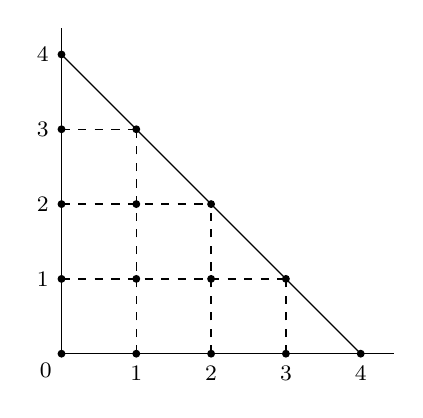
\begin{tikzpicture}[font=\footnotesize, line width=0.45pt, scale=0.95]
  % 坐标轴
  \draw (0,0) -- (4.45,0);
  \draw (0,0) -- (0,4.35);
  % 三角形边界（斜边）
  \draw (0,4) -- (4,0);
  % 三角形内的格线
  \begin{scope}
    \clip (0,0) -- (4,0) -- (0,4) -- cycle;
    \draw[dashed] (0,1) -- (4,1) (0,2) -- (4,2) (0,3) -- (4,3)
                  (1,0) -- (1,4) (2,0) -- (2,4) (3,0) -- (3,4);
  \end{scope}
  % 格点（共 15 个）
  \foreach \x in {0,...,4} {
    \foreach \y in {0,...,4} {
      \pgfmathparse{int(\x+\y<=4)}\ifnum\pgfmathresult=1
        \fill (\x,\y) circle (1.5pt);
      \fi
    }
  }
  % 刻度数字
  \foreach \x in {1,...,4} {
    \node[below] at (\x,-0.04) {$\x$};
  }
  \foreach \y in {1,...,4} {
    \node[left] at (-0.04,\y) {$\y$};
  }
  \node[below left] at (0,0) {$0$};
\end{tikzpicture}
\end{center}
\nopagebreak[4]
\begin{center}
\begin{tabular}{lllll}
\toprule
$X$ & $1$ & $2$ & $3$ & $4$ \\
\midrule
$Y$ & $51$ & $48$ & $45$ & $42$ \\
\bottomrule
\end{tabular}
\end{center}
这里，两株作物“相近”是指它们之间的直线距离不超过 $1$ 米。
（1） 完成下表，并求所种作物的平均年收获量；
\begin{center}
\begin{tabular}{lllll}
\toprule
$Y$ & $51$ & $48$ & $45$ & $42$ \\
\midrule
频数 &  & $4$ &  &  \\
\bottomrule
\end{tabular}
\end{center}
（2） 在所种作物中随机选取一株，求它的年收获量至少为 $48$ kg 的概率。
\end{question}
\begin{question}
\gkti{19}设 $S_n$ 为数列 $\{a_n\}$ 的前 $n$ 项和，已知 $a_1\ne0$，$2a_n-a_1=S_1\cdot S_n$，$n\in\mathbf N^*$。
（1） 求 $a_1$，$a_2$，并求数列 $\{a_n\}$ 的通项公式；
（2） 求数列 $\{na_n\}$ 的前 $n$ 项和。
\end{question}
\begin{question}
\gkti{20}已知 $F_1$，$F_2$ 分别是椭圆 $E:\dfrac{x^2}5+y^2=1$ 的左、右焦点，$F_1$，$F_2$ 关于直线 $x+y-2=0$ 的对称点是圆 $C$ 的一条直径的两个端点。
（1） 求圆 $C$ 的方程；
（2） 设过点 $F_2$ 的直线 $l$ 被椭圆 $E$ 和圆 $C$ 所截得的弦长分别为 $a$，$b$。当 $ab$ 最大时，求直线 $l$ 的方程。
\end{question}
\begin{question}
\gkti{21}已知函数 $f(x)=\dfrac{1-x}{1+x^2}\mathrm e^x$。
（1） 求 $f(x)$ 的单调区间；
（2） 证明：当 $f(x_1)=f(x_2)$（$x_1\ne x_2$）时，$x_1+x_2<0$。

\end{question}